\newpage
\section{Problem H - 传送带}
{ \limitfont{}
Input file: standard input \par
Output file: standard output \par
Time limit: 1000ms \par
Memory limit: 64MB \par
}
\subsection*{题目描述}
在一个空旷的地面上,dust把一些大小为1m * 1m的传送带组装成一个n行m列的矩形,如图所示
\begin{figure}[H]
    \centering
    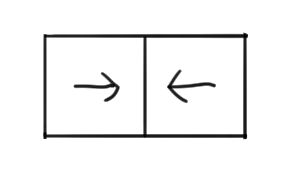
\includegraphics[scale=0.5]{./src/h.png}
\end{figure}
传送带一共有上下左右 $4$ 种传送方向,可以把在其上面的物品以 $1m/s$ 的速度沿其传送方向传送。

\textbf{输入保证传送带的方向一定指向其他传送带而不是空地}

dust 现把一个物品放到第 $x$ 行第 $y$ 列,问经过 $t$ 秒后该物品在第几行第几列
\subsection*{输入描述}
第一行两个整数 $n,m(2 \le n,m \le 10^3; n \times m \le 2 \times 10^5)$

下面 $n$ 行,每行 $m$ 个字母,其中第 $i$ 行的第 $j$ 个字母表示传送带的方向(' $U$ ',' $D$ ',' $L$ ',' $R$ '分别表示上下左右)

接下来一行一个整数 $q(1 \le q \le 2 \times 10^5)$,表示询问的次数

下面 $q$ 行,每行 $3$ 个整数 $x,y,t(1 \le x \le n,1 \le y \le m,1 \le t \le 10^{18})$
\subsection*{输出描述}

对于每次询问,输出一行两个整数,分别表示 $t$ 秒后该物品位置在第几行和第几列

\subsection*{测试样例}

\begin{table}[H]
\begin{tabularx}{\textwidth}{|X|X|}
    \hline
    \textbf{Standard Input} & \textbf{Standard Output} \\ 
    \hline 
    \tablecell{
        4 5 \\
        R R D D D \\
        D D R R D \\
        R U R U U \\
        U L L R U \\
        4 \\
        1 1 10 \\
        4 5 10 \\
        3 3 10 \\
        2 2 10 \\
    } & 
    \tablecell{3 5 \\
    2 5 \\
    3 5 \\
    2 2 \\ \\ \\ \\ \\ \\ \\} \\
    \hline
\end{tabularx}
\end{table}
